\chapter{Introduction}
\section{General}
The need for creating and generating synthetic or rather, data that is not real, has become a necessary factor in big companies. Some of the main reasons why such data is required to be created can be: privacy limitations, the need for test data, various experiments, research etc.\\
\newline
Synthetic data are generated to meet specific needs or certain conditions that may not be found in the original, real data. This can be useful when designing any type of system because the synthetic data are used as a simulation or as a theoretical value, situation, etc. This allows us to take into account unexpected results and have a basic solution or remedy, if the results prove to be unsatisfactory. Synthetic data are often generated to represent the authentic data and allows a baseline to be set. \cite{SyntheticDataUsefulness}\\
\newline
Business functions that usually benefit from the creation of synthetic data can be: Machine Learning, Data Mining, Agile Development, Researching etc. There are also several business types that benefit from synthetic data such as: Healthcare Systems, Financial Services, Fraud Detection Systems etc. \cite{AIMultipleSyntheticData}\\
\newline
At a first glance, synthetic data may seem like "random made up data", when in fact, behind that synthetic data, stand various algorithms and generation methods that are used to create such data which must look as realistic as possible.\\
Synthetic data is used mostly to protect the privacy and confidentiality of a particular set of data. Real data can contain personal information about people or things that a software engineer or researcher is not supposed to know. Therefore, synthetic data does not contain personal information that can fall into contrary with privacy laws or information that you can use to trace back to individuals.\\
\newline
There's often a misconception about Synthetic Data, Anonymized Data and Artificial Data. They serve mostly the same purposes but involve different techniques and results.\\ 
Anonymised Data is getting the original data and adding "noise" to it, encrypting it or even masking it. Ultimately, the anonymised data will correspond to the original data in some form somewhere.\\
Artificial Data on the other hand, is generated data with no linking or relation to original data apart from the model building.\\
\newline
In this project, we will be discussing the methods and techniques used for the generation of synthetic data and the original data used to generate such data, which means, fully artificial data with relation to the original data but with no clear signs of the original data.
\begin{figure}[H]
	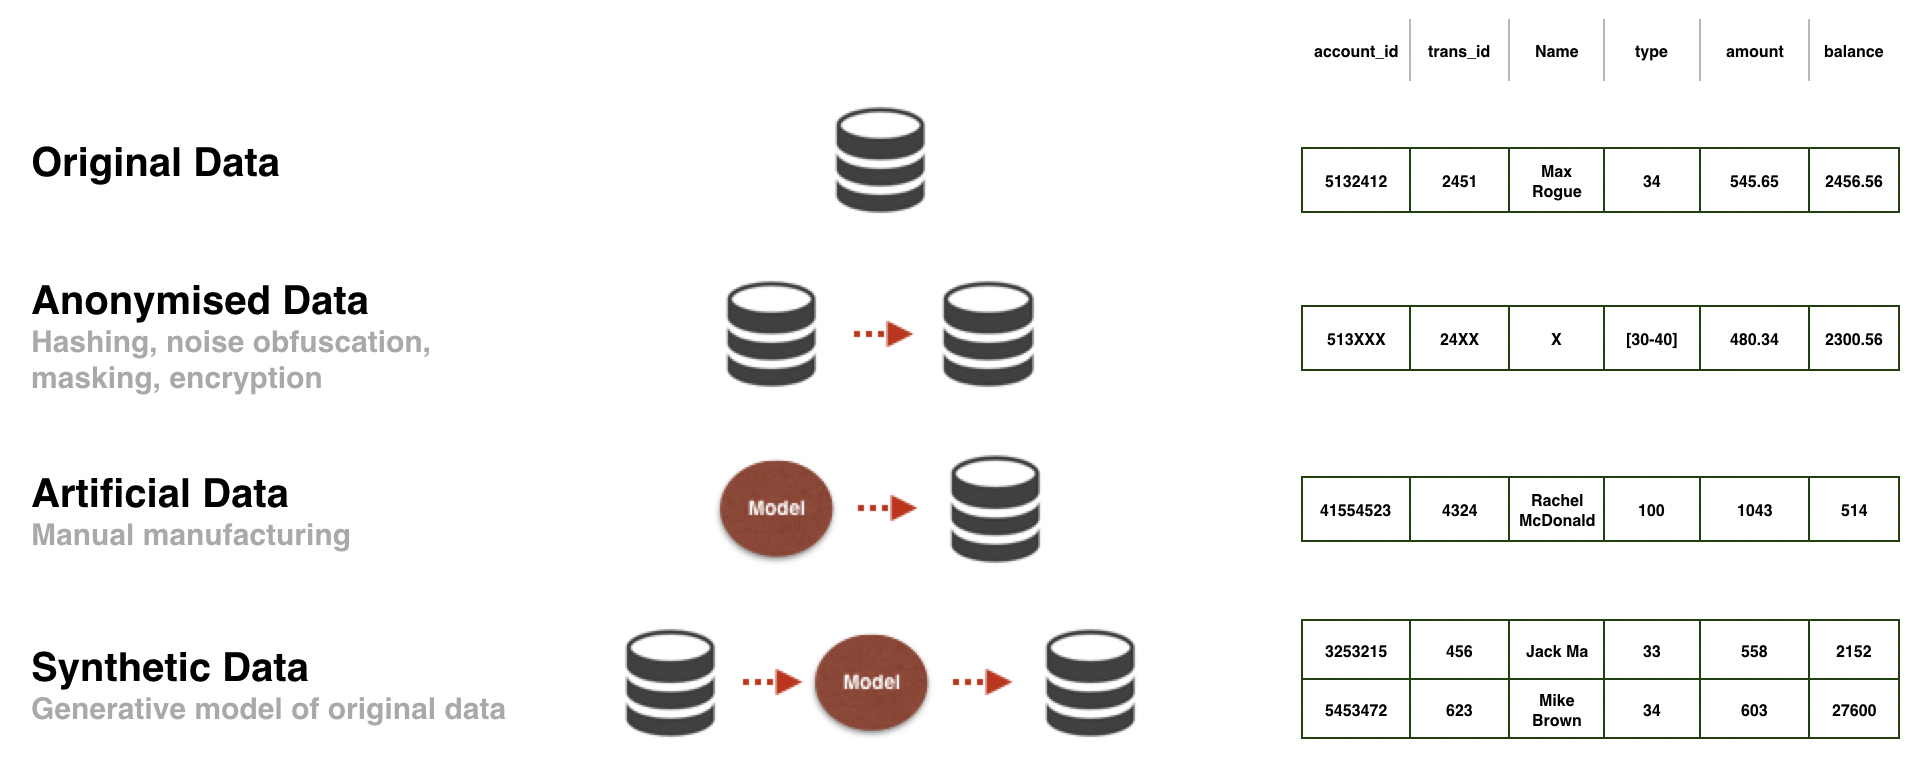
\includegraphics[width=\linewidth]{./Figures/Synthetic_Data/types_of_data_comparison.png}
	\caption{Three approaches to synthetic data, from \citeauthor{Synthesized_2018}}
\end{figure}
\section{Goals \& Requirements}
The main objective of this project is to successfully generate fully synthesized data that is as realistic as possible using the \textit{PostgreSQL} relational database management system and the \textit{Python} programming language in conjunction with some other third-party modules that mostly deal with numbers and mathematical functions.\\
\newline
This will be done using various methods and techniques that involve some sort of data anonymization, overcoming data type obstacles, histogram boundaries, respecting data privacy and data confidentiality etc. The tool initially tries to connect to an existing database and then based on the options provided, it will generate the synthesized data into a new desired database from the selected existing database. The process should be very straightforward.\\
\newline
The tool will be a single lightweight Python script that is executed from the shell terminal and which has various arguments that can be passed along with the command execution, with some of them being mandatory and some others optional (mostly related to database configuration and parameters).\\
It will initially connect to a PostgreSQL database (given with arguments) , read the \textit{pg\_class} table in order to obtain the tables of the given/accessed database and then fetch all the results of each table from the \textit{pg\_stats} table. 
To be continued...
\section{Synthetic Data Generation}
Synthetic data is a relatively new term for most of IT engineers. It has been emerging lately with the rise of applications and functions that require some sort of Machine Learning or Artifical Intelligence or just software engineers/QA who want to test their applications with a lot of data.\\
\newline
There exist a lot of ways for generating synthetic data and the languages/tools that are used to create such generation play a big role in defining the approach to generating such data. For example, here, PostgreSQL was used along with its \textit{pg\_stats} table and the whole tool relied on this table to do the synthetic data generation. Many other approaches exist and all of them have their advantages and disadvantages. The use for such data also has a very vast appliance and is very beneficial to the users that use it.\\
\newline
In this tool, a primary database with real data (or realistic) is required, the tool cannot generate anything without having the primary database to rely on and to gain information from and then manipulate that information to generate the synthetic data. A secondary database can exist (or the tool can create it itself) with the exact same schema as the primary database, however, the secondary database must be empty and truncated, ready for the synthetic data to be inserted into.\\
\newline
The synthetic data generation process involves a lot of mathematical functions, such as: randomization, probability, different mathematical distribution functions, frequencies etc. It also involves some manipulations with strings and this is done in order to achieve consistent and robust results when generating the synthetic data (The data exists in many forms).\\
A lot of mathematical Python libraries were used in this tool that contained necessary functions for the randomization and the generation of the synthetic data.
\section{Results}
Ultimately, the tool should generate fully synthetic data. This is displayed in this section by using some statistics about the database with the real/realistic data (primary database) and then some statistics for the synthesized database, which of course, contains the same schema as the primary one. It will display how similar the statistics about both of the databases are.\\
\newline
Statistics for the table \textit{atp\_players} of the primary database (with real data), as displayed in the \textit{pg\_stats} table (some numbers are rounded down in order to fit the table to the page):
\begin{table}[H]
\caption{Stats for the database with the real data}
\label{tab:real_data_stats}
\centering
\begin{tabularx}{\linewidth}{|l|r|X|r|X|X|X|}
\hline
	attname & null\_frac & avg\_width & n\_distinct & vals & freqs & bounds
	\\ \hline
hand          & 0.104533    & 2 & 3         & \{U,R,L\}                     & \{0.59, 0.28, 0.025\}        & null                                \\ \hline
player\_id    & 0           & 4 & -1        & null                          & null                              & \{100003, ... , 2009902\}           \\ \hline
last\_name    & 0.000766 & 8 & -0.540106 & \{Lee, Kim, ...\}        & \{0.00273, 0.00236, ...\}     & \{"A Cantacuzene", ... , "Zysset"\} \\ \hline
first\_name   & 0.00326  & 7 & -0.174477 & \{David, Daniel, ...\} & \{0.0105, 0.01, ...\}        & \{"A Baisley", ... ,  "Zygmunt"\}      \\ \hline
country\_code & 0.001       & 4 & 203       & \{USA, ESP, ...\}     & \{0.158867, 0.0478, 0.047667...\} & \{AFG, ... , ZAM\}                  \\ \hline
birth\_date   & 0.21196    & 4 & -0.240834 & \{19790525, 19870620, ...\}      & \{0.0003, 0.0003, 0.0003...\}     & \{18340000, ..., 20050210\}         \\ \hline
\end{tabularx}
\end{table}
\newpage
Statistics for the table \textit{atp\_players} of the generated database (with synthetic data), as displayed in the \textit{pg\_stats} table (some numbers are rounded down in order to fit the table to the page):
\begin{table}[H]
\caption{Stats for the database with the synthetic data}
\label{tab:synthetic_data_stats}
\centering
\begin{tabularx}{\linewidth}{|l|r|X|r|X|X|X|}
\hline
	attname & null\_frac & avg\_width & n\_distinct & vals & freqs & bounds
	\\ \hline
hand          & 0.107429    & 2 & 3         & \{F,A,G\}                     & \{0.59, 0.27, 0.025\}        & null                                \\ \hline
player\_id    & 0           & 4 & -1        & null                          & null                              & \{1, ... , 2746\}           \\ \hline
last\_name    & 0.0007283 & 8 & -0.876548 & \{Ukwfpqd, Oajhsjb, ...\}        & \{0.00619, 0.00546, ...\}     & \{"Aartxd", ... , "Zzxlbuj"\} \\ \hline
first\_name   & 0.0036416  & 7 & -0.634377 & \{Rdalbp, Sriyqz, ...\} & \{0.0127, 0.0076, ...\}        & \{"Abmydx", ... ,  "Zzylni"\}      \\ \hline
country\_code & 0.00072       & 4 & 128       & \{CIB, MSL, ...\}     & \{0.16169, 0.04879, 0.04878...\} & \{DWG, ... , YXR\}                  \\ \hline
birth\_date   & 0.217043    & 4 & -0.673343 & \{18765471, 19144610, ...\}      & \{0.0015, 0.0015, 0.0015...\}     & \{18340011, ..., 20048074\}         \\ \hline
\end{tabularx}
\end{table}
As displayed in the above tables, we can see that the similarity between the statistics is very high in the columns like: \textit{n\_distinct, avg\_width, most\_common\_vals, most\_common\_freqs} etc.\\
\newline
Only the \textit{n\_distinct} value is not similar because that can not be determined by the tool (only in the cases when it's positive) because since \textit{pg\_stats} table arrays only hold 100 values, we can't know the further frequencies of the other values and therefore cannot match the \textit{n\_distinct} of the real data.\\
\newline
More information on the \textit{pg\_stats} columns and their meanings can be found on the official PostgreSQL wiki page.